%\documentclass[article]{IEEEtran}
%\usepackage[utf8]{inputenc}
%\usepackage{graphicx}
%\usepackage{cite}
%\usepackage{url}

\title{GitHub Assignment}
\author{Noah Rodgers}
\date{September 2022}

%\begin{document}

\maketitle

\section{About Me}

Hello, my name is Noah Rodgers I am a Graduate Student in the Master of Cyber Security program at UCCS. I work at the Aerospace Corporation as an intern Cyber Specialist working with NASA and the Space Force. What I hope to gain from this course is how to properly conduct my research. As well as write my papers with the correct language and grammar. I hope this will further my research work as I start my work for Dr. Chang. I am working on disrupting satellite communications using different methods examining viability, and effectiveness. I am also hoping that this course will touch on how to write and prepare my thesis for my master’s program. Something personal about me is that I love to go sand boarding at the Great Sand dunes. I also like to long board to class from my home on sunny days although I’m not that good at it but I haven’t crashed yet, so I guess that’s a plus. I got my Bachelors in Game design and Development at UCCS and got my minor in computer science so I’ve been working on filling in the gaps for cyber security. I look forward to what this class has to offer.



\begin{figure}[!htb]
    \centering
    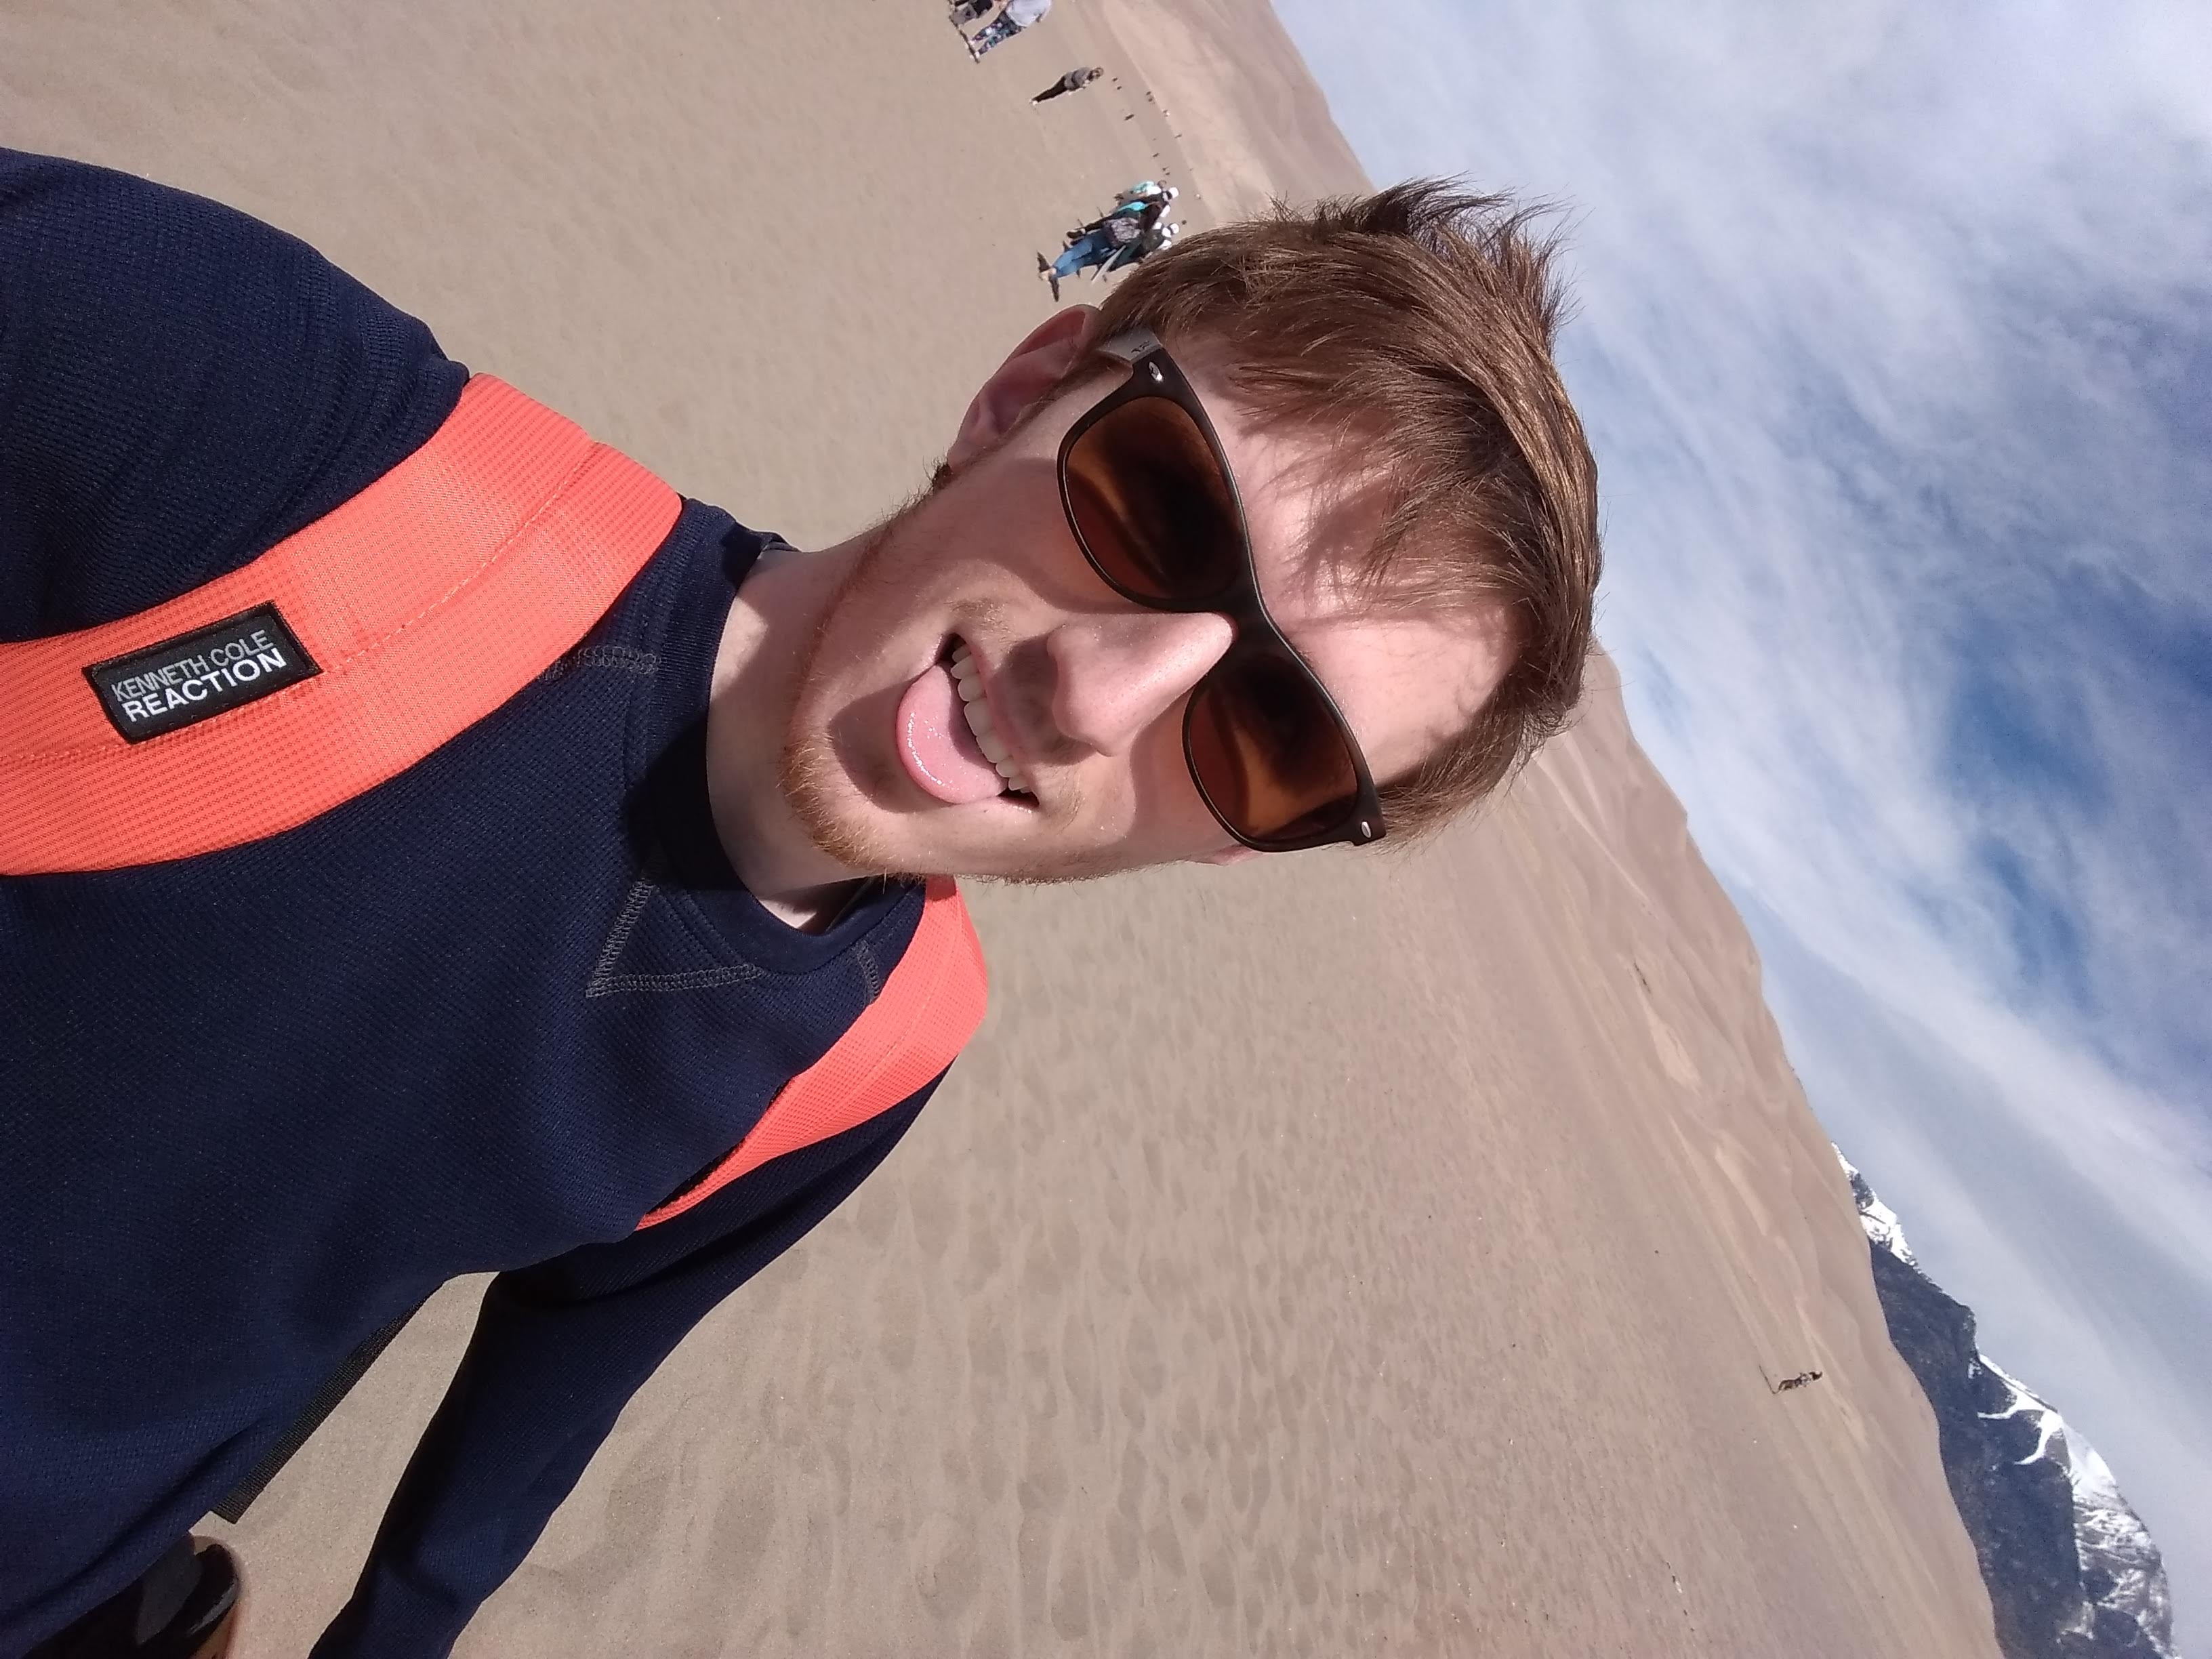
\includegraphics[width=85mm, angle=90]{Me1.jpg}
    \caption{\textbf{Picture of Myself}}
    \label{fig:jamequation}
\end{figure}


\section{Git Code}
A collection of Resources for budding SAT hackers (Satellites, not the test¯\_(ツ)_/¯).

This is the basic hack a sat github repo where you can learn and train to help better security for these devices.

https://github.com/deptofdefense/hack-a-sat-library

\section{2 Questions to answer}
How different is the attack vector when facing a hacking process aiming for satellites? - Jose Remy

Not very different although the problem we face in satellites is security vs time. Meaning that older satellites are still up above us floating around still being used for missions and for everyday use. This saves money when we can jsut reuse whats up there already but faces the problem of these systems, these languages they use, the interfaces, their ancient in some terms. Satallite attacks are much like the internet built for acceibility and use rather than security so we see alot of the same attack vectors as any other that would be used.



\bibliographystyle{IEEEtran}
\bibliography{refs}

%\end{document}
